% coding:utf-8

\section{Recoveryzeit}

\subsection{Messaufbau}
\begin{frame}
Bild
%   \begin{figure}
%     \includegraphics[width=1.0\columnwidth]{fig/ti_ds_dco_freq.pdf}
%     \caption{Auszug aus dem Datenblatt des MSP430G2553}
%   \end{figure}
\end{frame}

\subsection{Erwartung}
\begin{frame}
  \begin{itemize}
    \item 1N4007 relativ langsam
    \item 1N4148 schneller
    \item BAT81 noch schneller
  \end{itemize}
\end{frame}

\subsection{Ergebnisse}
\subsubsection{1N4007}
\begin{frame}
  \begin{figure}
    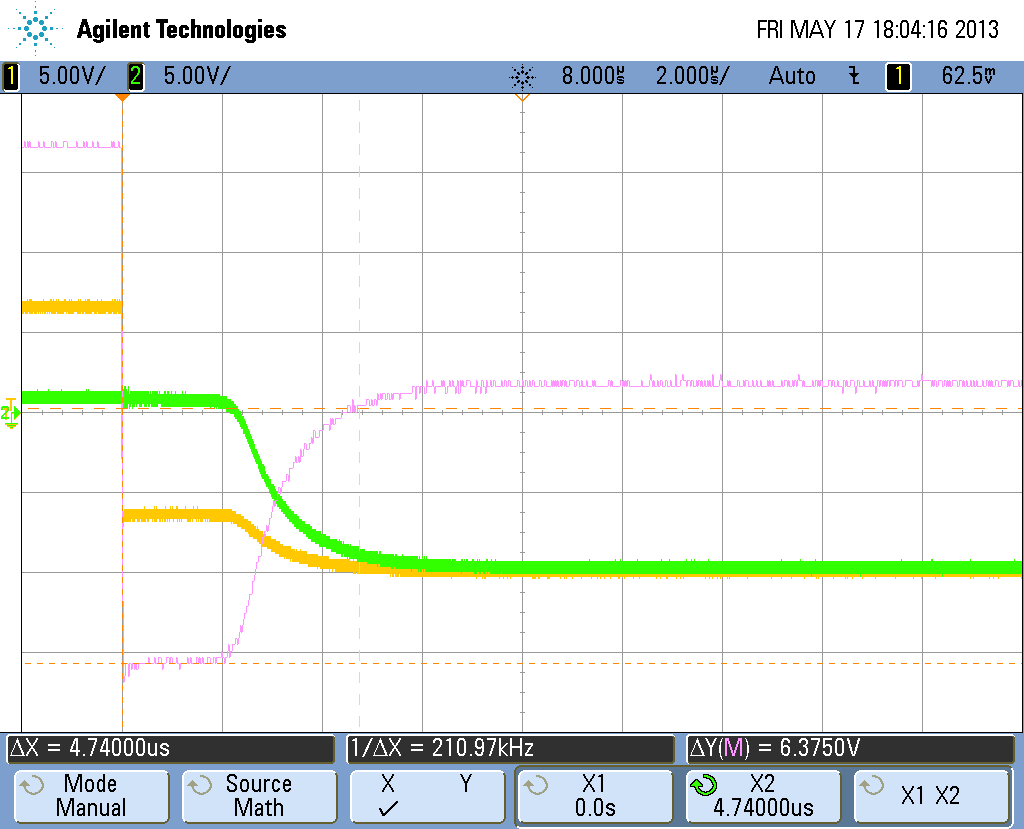
\includegraphics[width=1.0\columnwidth]{fig/scope_18.png}
    \caption{1N4007}
  \end{figure}
\end{frame}

\subsubsection{1N4148}
\begin{frame}
  \begin{figure}
    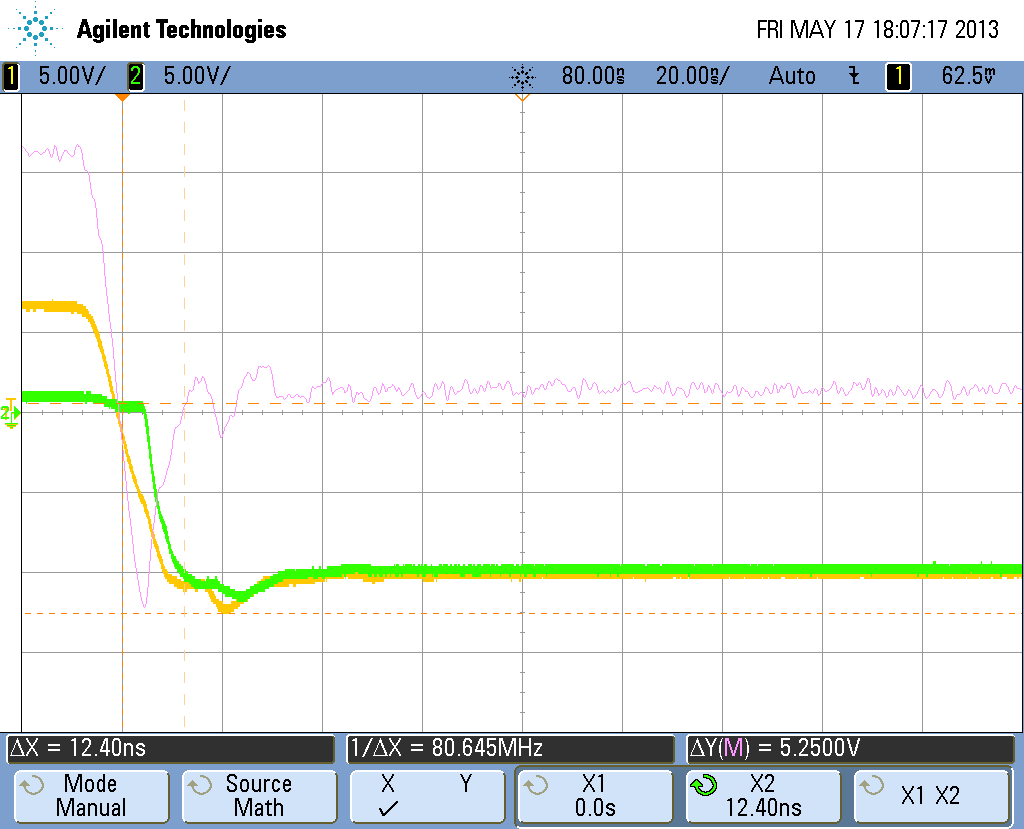
\includegraphics[width=1.0\columnwidth]{fig/scope_19.png}
    \caption{1N4148}
  \end{figure}
\end{frame}

% \subsection{BAT81}
% \begin{frame}
%   \begin{figure}
%     \includegraphics[width=1.0\columnwidth]{fig/scope_20.png}
%     \caption{BAT81}
%   \end{figure}
% \end{frame}
